\chapter{Passeio do CG}
\label{passeioCG}
O passeio do centro de gravidade (CG) da aeronave foi realizado conforme metodologia proposta por Gudmundsson \cite{gudmundsson} e esta estabelece, conforme o requisito do regulamento de que a aeronave deve ser estável, que o centro de gravidade da aeronave deve permanecer dentro de alguns limites pré-estabelecidos. A localização do centro de gravidade da aeronave é um parâmetro de extrema importância para o piloto e é responsabilidade da companhia assegurar que a aeronave está carregada de maneira que o centro de gravidade permaneça dentro do limite do envelope permitido durante todo o voo.

Durante o cálculo do envelope do centro de gravidade, foi estabelecida que o ponto de referência (0,0,0) estivesse na frente e abaixo do nariz da aeronave. Isto, conforme  Gudmundsson \cite{gudmundsson}, assegura que os momentos calculados devidos aos pesos dos componentes, passageiros e outros carregamentos, possuam somente um sinal, evitando a chance da ocorrência de erros matemáticos. Há dois métodos de indicar a localização do CG da aeronave, em termos da porcentagem da corda média geométrica ou em termos das estações da fuselagem, e para este trabalho foi escolhido indicar da primeira forma.

Durante o projeto de uma aeronave, a determinação do centro de gravidade da mesma é um passo necessário e crucial, sendo que o principal motivo é para determinar os
limites dianteiros e traseiros que garantam a operação segura da aeronave. Conforme proposto na bibliografia adotada, determinou-se a nuvem de passeio do centro de gravidade, mostrada na \autoref{fig:passeioCG}, que consiste nas diversas combinações de passageiros e seus posicionamentos, bagagens e combustível na aeronave. Utilizou-se os dados das estimativas dos pesos dos componentes e dos diversos sistemas que compõem a aeronave para estimar o centro de gravidade da aeronave vazia. A \autoref{tbl:cg_vazio} apresenta os dados utilizados para a obtenção do centro de gravidade da aeronave vazia em que posição do CG de cada componente é medida em relação ao nariz do avião.

\clearpage

\begin{table}[H]
\centering
\begin{tabular}{ccccc}
\toprule
 Componente & Peso (lbf) & Peso (kgf) & Posição CG & Momento (N$\cdot$m) \\ \midrule
Asa & 3164.2 & 1435.3 & 14.3 & 200710.6 \\
Empenagem Horizontal & 161.5 & 73.3 & 27.8 & 19945.9 \\
Empenagem Vertical & 263.6 & 119.6 & 27.8 & 32555.6 \\
Fuselagem & 3105.4 & 1408.6 & 11.0 & 152278.4 \\
Trem de Pouso Principal & 1023.7 & 464.3 & 14.3 & 64935.0 \\
Trem de Pouso de Nariz & 225.4 & 102.2 & 2.2 & 2166.4 \\
Sistema Propulsivo & 3171.8 & 1438.7 & 14.3 & 201192.7 \\
Sistema de Combustível & 628.8 & 285.2 & 14.3 & 39885.8 \\
Sistema de Controle & 1708.5 & 775.0 & 2.2 & 16421.3 \\
Sistema Hidráulico & 46.5 & 21.1 & 16.2 & 3356.7 \\
Sistema de Ar Condicionado & 3517.6 & 1595.6 & 14.3 & 223127.4 \\
Sistema Elétrico & 769.8 & 361.4 & 13.5 & 47865.5 \\
Sistema de Aviônicos & 2786.5 & 1263.9 & 13.4 & 166151.0 \\
Acessórios & 205.7 & 93.3 & 18.0 & 16475.8 \\
APU & 154.322 & 70.0 & 29 & 19914.3 \\
\bottomrule
\end{tabular}
\caption{Obtenção do CG da aeronave vazia}
\label{tbl:cg_vazio}
\end{table}.

Obteve-se o seguinte resultado para o centro de gravidade da aeronave vazia.

\begin{table}[H]
\centering
\begin{tabular}{cccc}
\toprule
 Massa total (kg) & Peso vazio total (N) & Momento (N$\cdot$m) & Posição CG  \\ \midrule
9507.5 & 93269.0 & 1206982.5 & 12.9 \\
\bottomrule
\end{tabular}
\caption{CG da aeronave vazia}
\label{tbl:cg_vazio_res}
\end{table}.

Posteriormente, os passageiros foram adicionados um a um, partindo da posição dos assentos mais dianteira até a mais traseira e depois da mais traseira a mais dianteira, conforme apresentado na tabela do passeio do centro de gravidade que está em anexo, e obteve-se o passeio mostrado na \autoref{fig:passeioCG}. Portanto, essa nuvem de dados fornece os limites das posições do centro de gravidade para uma operação segura da aeronave.

\clearpage

\begin{figure}[H]
\centering
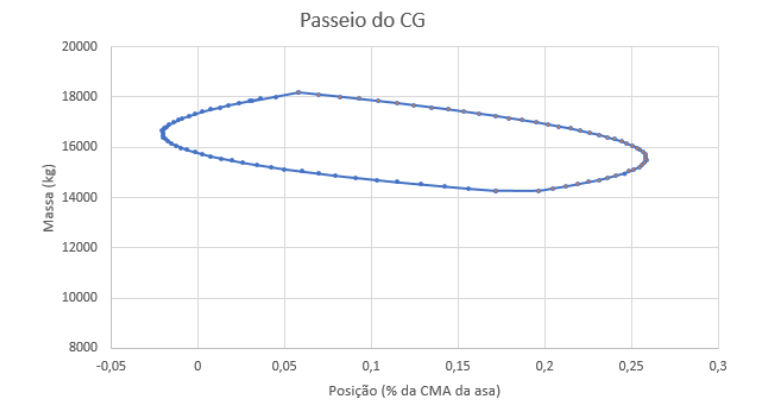
\includegraphics[width=0.85\textwidth]{images/parte3/passeioCG.PNG}
\caption{Passeio do CG}
\label{fig:passeioCG}
\end{figure}

Como observado no gráfico e com os resultados apresentados na tabela do passeio do CG que se encontra no anexo, os limites do passeio do centro de gravidade são os seguintes:


\begin{table}[H]
\centering
\begin{tabular}{ccc}
\toprule
 Posição: & Em relação ao nariz & Em \% da CMA  \\ \midrule
 Limite Dianteiro & 13.5 m & -2.0\% \\
 Limite Traseiro & 14.3 m & 25.8\% \\
\bottomrule
\end{tabular}
\caption{Limites do passeio do centro de gravidade}
\label{tbl:cg_limites}
\end{table}.

\clearpage
